\chapter{Pivoting}

In the last lecture, we saw that Gaussian elimination in its pure form is unstable. The instability can be controlled by permuting the order of the rows of the matrix being operated on, an operation called pivoting. Pivoting has been a standard feature of Gaussian elimination computations since the 1950s. 

\section{Pivots}
At step $k$ of Gaussian elimination, multiples of row $k$ are subtracted from rows $k+1, \ldots, m$ of the working matrix $X$ in order to introduce zeros in entry $k$ of these rows. In this operation row $k$, column $k$, and especially the entry $x_{k k}$ play special roles. We call $x_{k k}$ the \textbf{pivot}. From every entry in the submatrix $X_{k+1: m, k: m}$ is subtracted the product of a number in row $k$ and a number in column $k$, divided by $x_{k k}$:
%────────────────────────────────────────
\begin{figure}[H]
    \centering
    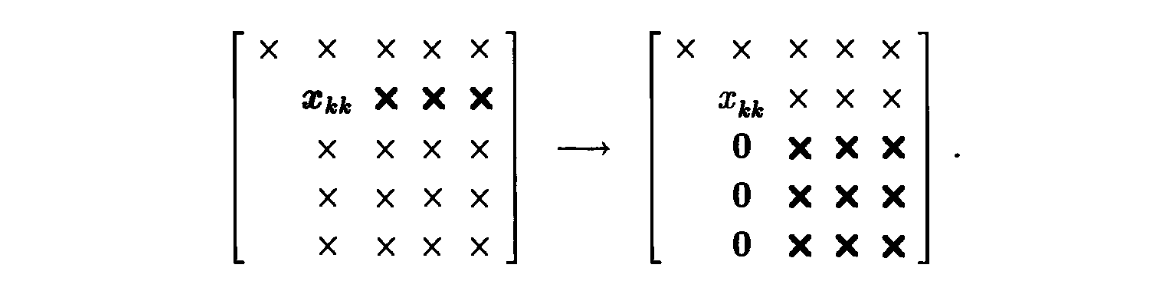
\includegraphics[width=0.8\textwidth]{figures/21-1.png}
\end{figure}
%────────────────────────────────────────
However, we don't really have to choose $x_{kk}$ as the pivot. We can also choose $x_{ik}$: 

%────────────────────────────────────────
\begin{figure}[H]
    \centering
    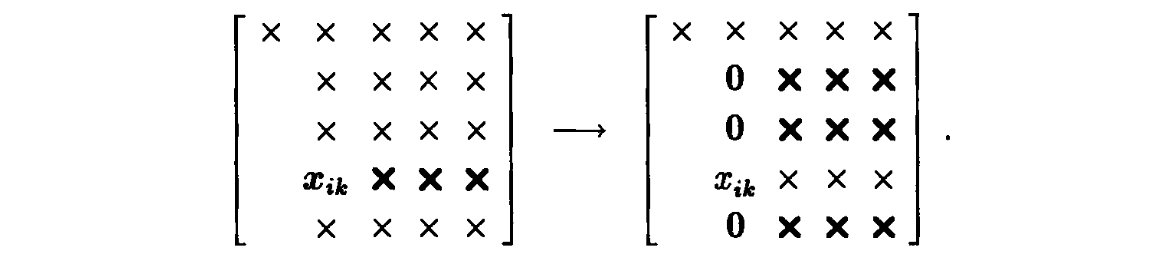
\includegraphics[width=0.8\textwidth]{figures/21-2.png}
\end{figure}
%────────────────────────────────────────
Similarly, we can also introduce zeros in column $j$ rather than column $k$:
%────────────────────────────────────────
\begin{figure}[H]
    \centering
    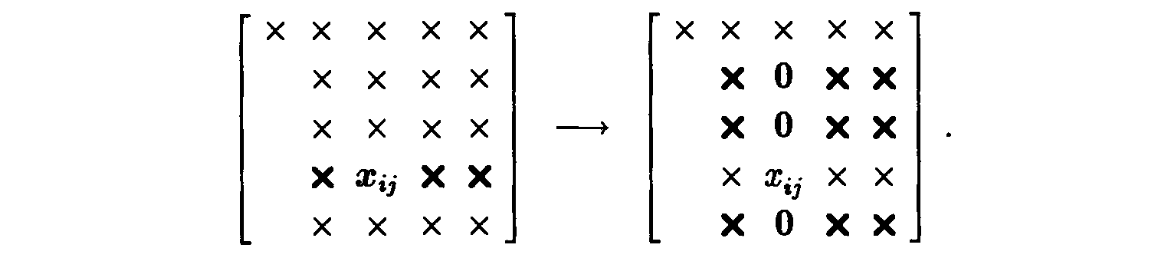
\includegraphics[width=0.8\textwidth]{figures/21-3.png}
\end{figure}
%────────────────────────────────────────
All in all, we are free to choose any entry of $X_{k:m, k:m}$ as the pivot, as long as it's nonzero. For numerical stability, it's desirable to pivot even when $x_{kk}$ is nonzero if there is a larger element available. In practice, we just pick as pivot the largest number among a set of entries. Now at step $k$, we will permute the rows and columns to make $x_{kk}$ is the largest number. This interchange of rows and perhaps columns is what is usually thought of as \textbf{pivoting}.  


%────────────────────────────────────────
\begin{note}
The ideal that rows and columns are interchanged is indispensable conceptually. Whether it's a good idea to interchange them physically on the computer is less clear. In some implementations, the data in computer memory are indeed swapped at each pivot step. In others, an equivalent effect is achieved by indirect addressing with permuted index vectors. Which is best varies from machine to machine and depends on many factors. 
\end{note}
%────────────────────────────────────────

\section{Partial Pivoting}
If every entry of $X_{k:m, k:m}$ is considered as a possible pivot at step $k$, there are $O((m-k)^2)$ entries to be examined to determine the largest. Summing over $m$ steps, the total cost of selecting pivots is $O(m^3)$, adding significant to the cost of Gaussian elimination. This expensive strategy is called \textbf{complete pivoting}. 

In practice, we only interchange rows and this standard method is called the \textbf{partial pivoting}. The pivot at each step is chosen as the largest of the $m-k+1$ subdiagonal entries in column $k$, incurring a total cost of only $O(m^2)$ operations.  
%────────────────────────────────────────
\begin{figure}[H]
    \centering
    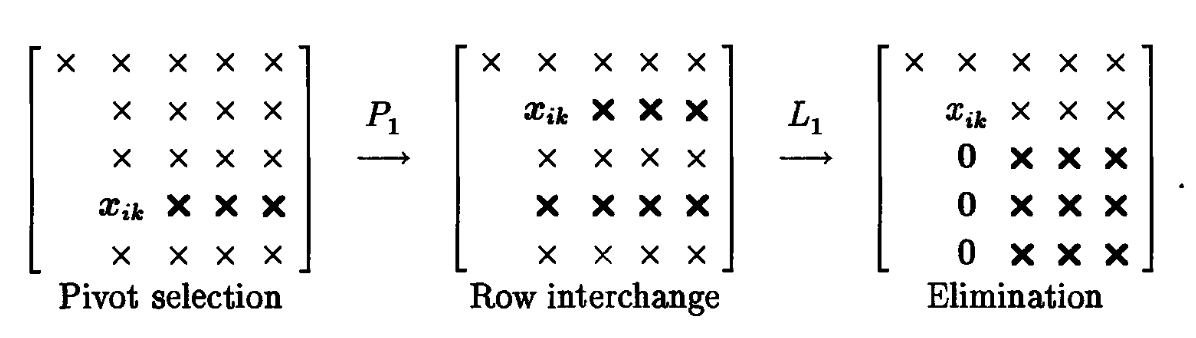
\includegraphics[width=0.8\textwidth]{figures/21-4.png}
\end{figure}
%────────────────────────────────────────
This algorithm can be expressed as a matrix product. Now we need some permutation matrices $P_k$. After $m-1$ steps, $A$ becomes an upper-triangular matrix $U$: 
\begin{equation}
\label{eq: pivot C}
L_{m-1} P_{m-1} \cdots L_2 P_2 L_1 P_1 A=U. 
\end{equation}

\section{Example}
Let's return to the example we already checked: 
\[
    A = \begin{bmatrix}
        2 & 1 & 1 &  0 \\
        4 & 3 & 3 &  1 \\
        8 & 7 & 9 &  5 \\
        6 & 7 & 9 &  8 \\
    \end{bmatrix}.  
\]
The first pivoting $P_1$: 
\[
    \begin{bmatrix}
         &  & 1 &   \\
         & 1 &  &   \\
        1 &  &  &   \\
         &  &  &  1 \\
    \end{bmatrix} 
    \begin{bmatrix}
        2 & 1 & 1 &  0 \\
        4 & 3 & 3 &  1 \\
        8 & 7 & 9 &  5 \\
        6 & 7 & 9 &  8 \\
    \end{bmatrix}
    = 
    \begin{bmatrix}
        8 & 7 & 9 &  5 \\
        4 & 3 & 3 &  1 \\
        2 & 1 & 1 &  0 \\
        6 & 7 & 9 &  8 \\
    \end{bmatrix}. 
\]
The first elimination step now is $L_1$: 
\[
    \begin{bmatrix}[1.3]
        1 &  &  &   \\
        -\frac{1}{2} & 1 &  &   \\
        -\frac{1}{4} &  &1   &   \\
         -\frac{3}{4} &  &  &1   \\
    \end{bmatrix} 
    \begin{bmatrix}[1.3]
        8 & 7 & 9 &  5 \\
        4 & 3 & 3 &  1 \\
        2 & 1 & 1 &  0 \\
        6 & 7 & 9 &  8 \\
    \end{bmatrix} 
    = 
    \begin{bmatrix}[1.3]
        8 & 7 & 9 &  5 \\
         & -\frac{1}{2} & -\frac{3}{2} &  -\frac{3}{2} \\
         & -\frac{3}{4} & -\frac{5}{4} &  -\frac{5}{4} \\
         & -\frac{7}{4} & -\frac{9}{4} &  \frac{17}{4} \\
    \end{bmatrix}.  
\]
Now the second the forth rows are interchanged $P_2$: 
\[
    \begin{bmatrix}[1.3]
        1 &  &  &   \\
         &  &  &  1 \\
         &  & 1 &   \\
         & 1 &  &   \\
    \end{bmatrix}  
    \begin{bmatrix}[1.3]
        8 & 7 & 9 &  5 \\
         & -\frac{1}{2} & -\frac{3}{2} &  -\frac{3}{2} \\
         & -\frac{3}{4} & -\frac{5}{4} &  -\frac{5}{4} \\
         & \frac{7}{4} & \frac{9}{4} &  \frac{17}{4} \\
    \end{bmatrix}
    = 
    \begin{bmatrix}[1.3]
        8 & 7 & 9 &  5 \\
        & \frac{7}{4} & \frac{9}{4} &  \frac{17}{4} \\
         & -\frac{1}{2} & -\frac{3}{2} &  -\frac{3}{2} \\
         & -\frac{3}{4} & -\frac{5}{4} &  -\frac{5}{4} \\
    \end{bmatrix}
    .
\]
Then we do the second elimination step $L_2$. 
\[
    \begin{bmatrix}[1.3] 
        1 &  &  &   \\
         & 1 &  &   \\
         & \frac{3}{7} & 1 &   \\
         & \frac{2}{7} &  &  1 \\
    \end{bmatrix} \begin{bmatrix}[1.3] 
        8 & 7 & 9 &  5 \\
         & \frac{7}{4} & \frac{9}{4} &  \frac{17}{4} \\
         & -\frac{3}{4} & -\frac{5}{4} &  -\frac{5}{4} \\
         & -\frac{1}{2} & -\frac{3}{2} &  -\frac{3}{2} \\
    \end{bmatrix} = 
    \begin{bmatrix}[1.3] 
        8 & 7 & 9 &  5 \\
         & \frac{7}{4} & \frac{9}{4} &  \frac{17}{4} \\
         &  & -\frac{2}{7} &  \frac{4}{7} \\
         &  & -\frac{6}{7} &  -\frac{2}{7} \\
    \end{bmatrix}. 
\]
Now we change the third and the fourth rows $P_3$: 
\[
    \begin{bmatrix}[1.3] 
        1 &  &  &   \\
         & 1 &  &   \\
         &  &  &  1 \\
         &  & 1 &   \\
    \end{bmatrix}
    \begin{bmatrix}[1.3] 
        8 & 7 & 9 &  5 \\
         & \frac{7}{4} & \frac{9}{4} &  \frac{17}{4} \\
         &  & -\frac{2}{7} &  \frac{4}{7} \\
         &  & -\frac{6}{7} &  -\frac{2}{7} \\
    \end{bmatrix}. 
    = 
    \begin{bmatrix}[1.3] 
        8 & 7 & 9 &  5 \\
         & \frac{7}{4} & \frac{9}{4} &  \frac{17}{4} \\
         &  & -\frac{6}{7} & -\frac{2}{7}   \\
         &  &-\frac{2}{7}  & \frac{4}{7}   \\
    \end{bmatrix}  . 
\]

The final step $(L_3)$ is: 
\[
    \begin{bmatrix}[1.3] 
       1  &  &  &   \\
         & 1 &  &   \\
         &  & 1&   \\
         &  & -\frac{1}{3} &1   \\
    \end{bmatrix}  
    \begin{bmatrix}[1.3] 
        8 & 7 & 9 &  5 \\
         & \frac{7}{4} & \frac{9}{4} &  \frac{17}{4} \\
         &  & -\frac{6}{7} & -\frac{2}{7}   \\
         &  &-\frac{2}{7}  & \frac{4}{7}   \\
    \end{bmatrix}  
    = 
    \begin{bmatrix}[1.3] 
        8 & 7 & 9 &  5 \\
         & \frac{7}{4} & \frac{9}{4} &  \frac{17}{4} \\
         &  & -\frac{6}{7} &  -\frac{2}{7} \\
         &  &  &  \frac{2}{3} \\
    \end{bmatrix}.  
\]

\section{$ PA=LU $ Factorization and a Third Stroke of Luck}
However, we are not doing LU but get an LU of $PA$, where $P$ is a permutation matrix. Combine all of them, it looks like: 
\[
    \begin{bmatrix}[1.3] 
         &  & 1 &   \\
         &  &  &  1 \\
         & 1 &  &   \\
        1 &  &  &   \\
    \end{bmatrix} 
    \begin{bmatrix}[1.3] 
        2 & 1 & 1 &  0 \\
        4 & 3 & 3 &  1 \\
        8 & 7 & 9 &  5 \\
        6 & 7 & 8 &  9 \\
    \end{bmatrix}
    = 
    \begin{bmatrix}[1.3] 
        1 &  &  &   \\
        -\frac{3}{4} & 1 &  &   \\
        \frac{1}{2} & -\frac{2}{7} & 1 &   \\
        \frac{1}{4} & -\frac{3}{7} & \frac{1}{3} &  1 \\
    \end{bmatrix}
    \begin{bmatrix}[1.3] 
        8 & 7 & 9 &  5 \\
         & \frac{7}{4} & \frac{9}{4} &  \frac{17}{4} \\
         &  & -\frac{6}{7} &  -\frac{2}{7}  \\
         &  &  &  \frac{2}{3}   \\
    \end{bmatrix}   . 
\]
Note that, all the subdiagonal entries of $L$ are smaller than $1$. Our elimination process took the form: 
\[
    L_3P_3 L_2 P_2 L_1 P_1 A = U, 
\]
which doesn't look lower-traingular at all. However, a third stroke of good fortune has come to our aid. The sec elementary operations can be reordered in the form 
\[
    L_3P_3 L_2 P_2 L_1 P_1 = L_3' L_2' L_1' P_3 P_2 P_1, 
\]
where $L_k^{\prime}$ is equal to $L_k$ but with the subdiagonal entries permuted. To be precise, define
$$
L_3^{\prime}=L_3, \quad L_2^{\prime}=P_3 L_2 P_3^{-1}, \quad L_1^{\prime}=P_3 P_2 L_1 P_2^{-1} P_3^{-1}
$$

Since of these definitions applies only permutations $P_j$ with $j>k$ to $L_k$, it's easily verified that $L_k'$ has the same structure as $L_k$.


In general, for an $m \times m$ matrix, the factorization provided by Gaussian elimination with partial pivoting can be written in the form
$$
\left(L_{m-1}^{\prime} \cdots L_2^{\prime} L_1^{\prime}\right)\left(P_{m-1} \cdots P_2 P_1\right) A=U,
$$
where $L_k^{\prime}$ is defined by
$$
L_k^{\prime}=P_{m-1} \cdots P_{k+1} L_k P_{k+1}^{-1} \cdots P_{m-1}^{-1}
$$

The product of the matrices $L_k'$ is unit lower-triangular and easily invertible by negating the subdiagonal entries, just as in Gaussian elimination without pivoting. Writing $ L= (L'_{m-1}\cdots L_2' L_1')^{-1}  $  and $P=P_{m-1}\cdots P_2 P_1$, we have 
\begin{equation}
\label{eq: pivot LU}
    PA = LU. 
\end{equation}

In general, any square matrix $A$, singular or nonsingular, has a factorization \eqref{eq: pivot LU}, where $P$ is a permutation matrix, $L$ is unit lower-triangular with lower-triangular entries $\leq 1$ in magnitude, and $U$ is upper-triangular. Partial pivoting is such a universal practice that this factorization is usually known simply as an \textbf{LU factorization} of $A$. This formula has a simple interpretation. 
\begin{itemize}
    \item Permute the rows of $A$ according to $P$,
    \item Apply Gaussian elimination without pivoting to $PA$. 
\end{itemize}

The algorithm of LU with partial pivoting is: 

\begin{algorithm}[H]
    \caption{Gaussian Elimination with Partial Pivoting}
    \label{Algo 21.1}
    $ U=A, L=I, P=I $\; 
    \For{$ k=1 $ \KwTo $ m-1 $ }{
        Select $ i\ge k $ to maximize $ |u_{ik}| $\; 
        $ u_{k,k:m} \leftrightarrow u_{i,k:m} $ (interchange two rows)\; 
        $ l_{k,1:k-1} \leftrightarrow l_{i, 1:k-1} $ \; 
        $ p_{k,:} \leftrightarrow p_{i,:} $ \; 
        \For{$ j=k+1 $ \KwTo $ m $ } {
            $ l_{jk} = u_{jk}/u_{kk} $\; 
            $ u_{j,k:m}  = u_{j,k:m} - l_{jk}u_{k,k:m}$  
        }
    } 
\end{algorithm}

Note that the $L_k = I - v_k e_k^*$, hence 
\begin{align*}
    L_k' = I + P_{m-1} \cdots P_{k+1} (I+ v_k e_k^*) P_{k+1}^{-1} \cdots P_{m-1}^{-1} &= I - P_{m-1} \cdots P_{k+1} v_k e_k^* P_{k+1}^{-1} \cdots P_{m-1}^{-1}\\ 
    &= I-P_{m-1} \cdots P_{k+1} v_k e_k^*.     
\end{align*}
Hence, we have 
\[
    (L_k')^{^{-1} } = I - P_{m-1} \cdots P_{k+1} v_k e_k^*. 
\]
This explains why we can update $L$ like this in the algorithm. 

To leading order, this algorithm requires the same number of floating point operations as Gaussian elimination without pivoting, namely, $\frac{2}{3} m^3$. As with \autoref{Algo 20.1}, the use of computer memory can be minimized if desired by overwriting $U$ and $L$ into the same array used to store $A$.

In practice, of course, $P$ is not represented explicitly as a matrix. The rows are swapped at each step, or an equivalent effect is achieved via a permutation vector, as indicated earlier.

\section{Complete Pivoting}
In complete pivoting, the selection of pivots takes a significant amount of time. In practice this is rarely done, because the improvement in stability is marginal. However, we shall outline how the algebra changes in this case.

In matrix form, complete pivoting precedes each elimination step with a permutation $P_k$ of the rows applied on the left and also a permutation $Q_k$ of the columns applied on the right:
$$
L_{m-1} P_{m-1} \cdots L_2 P_2 L_1 P_1 A Q_1 Q_2 \cdots Q_{m-1}=U .
$$
Once again, this is not quite an LU factorization of $A$, but it is close. If the $L_k^{\prime}$ are defined as the partial pivoting (the column permutations are not involved), then
$$
\left(L_{m-1}^{\prime} \cdots L_2^{\prime} L_1^{\prime}\right)\left(P_{m-1} \cdots P_2 P_1\right) A\left(Q_1 Q_2 \cdots Q_{m-1}\right)=U \text {. }
$$
Setting $L=\left(L_{m-1}^{\prime} \cdots L_2^{\prime} L_1^{\prime}\right)^{-1}, P=P_{m-1} \cdots P_2 P_1$, and $Q=Q_1 Q_2 \cdots Q_{m-1}$, we obtain
$$
P A Q=L U.
$$